\documentclass[../TDO4.tex]{subfiles}%

\begin{document}
\section[s]"3"{Lunettes astronomiques de Kepler et Galilée}
\enonce{%
	On construit une lunette astronomique de Kepler par un objectif $\Lc_1$ de
	diamètre $D = \SI{30}{mm}$, de centre O$_1$ et de vergence $V_1 =
		\SI{3.125}{\delta}$, et d'un oculaire $\Lc_2$ de centre $O_2$ et de vergence
	$V_2 = \SI{25}{\delta}$.
}%

\subsection{Kepler}
\ifcorrige{%
	\begin{center}
		\begin{tcn}(data){Données}
			Association de deux lentilles~:
			\begin{enumerate}
				\item $\Lc_1$ « objectif », vergence $V_1 = \SI{3.125}{\de}$, diamètre $D
					      = \SI{30}{mm}$ ;
				\item $\Lc_2$ « oculaire », vergence $V_2 = \SI{25}{\de}$.
			\end{enumerate}
		\end{tcn}
	\end{center}
}%

\QR{%
	Calculer les distances focales images $f'_1$ et $f'_2$ de l'objectif
	et de l'oculaire respectivement.
}{%
	~
	\begin{tcbraster}[raster columns=7, raster equal height=rows]
		\begin{tcn}[raster multicolumn=2](ques){Résultat attendu}
			Focales de lentilles
		\end{tcn}
		\begin{tcn}[raster multicolumn=2](tool)""{Outil du cours}
			\[
				V = \dfrac{1}{f'}
			\]
		\end{tcn}
		\begin{tcn}[raster multicolumn=3, valign=top](appl)'r'{Application}
			\[
				\xul{\obarr{O_1F'_1} = \SI{32}{cm}}
				\qet
				\xul{\obarr{O_2F'_2} = \SI{4}{cm}}
			\]
		\end{tcn}
	\end{tcbraster}
}%

\QR{%
	Définir le caractère afocal d'une lunette et son intérêt pour un
	œil emmétrope.
}{%
	~
	\begin{tcbraster}[raster columns=2, raster equal height=rows]
		\begin{tcn}(data){Système afocal}
			Est afocal un système pour lequel un objet initial à l'infini donne une
			image finale à l'infini.
		\end{tcn}
		\begin{tcn}*(inte)"left"'r'{Intérêt d'un système afocal}
			Un système afocal présente comme intérêt de permettre à un œil emmétrope
			d'observer sans fatigue, étant donné que l'image sortant du système est à
			l'infini (voir cours).
		\end{tcn}
	\end{tcbraster}
}%

\QR{\label{q:k_encomb}%
	Calculer alors l'encombrement $\obarr{O_1O_2}$ de la lunette.
}{%
	~
	\begin{tcbraster}[raster columns=7, raster equal height=rows]
		\begin{tcolorbox}[blankest, raster multicolumn=3, space to=\myspac]
			\begin{tcbraster}[raster columns=1]
				\begin{tcn}[](ques){Résultat attendu}
					$$\obarr{O_1O_2}$$
				\end{tcn}
				\begin{tcn}[add to natural height=\myspac](tool){Outils du cours}
					Règles de construction de rayons~:
					\begin{enumerate}
						\item Un rayon provenant de l'infini émerge d'une lentille en
						      croisant l'axe optique au plan focal image ;
						\item Des rayons se croisant dans le plan focal objet d'une lentille
						      émergent parallèles entre eux.
					\end{enumerate}
					Composition des distances~:
					\[
						\obarr{O_1O_2} = \obarr{O_1F_1'} + \obarr{F_1'O_2}
					\]
				\end{tcn}
			\end{tcbraster}
		\end{tcolorbox}
		\begin{tcn}[raster multicolumn=4](appl)'r'{Application}
			Pour que tous les rayons sortant de la lunette soient parallèles entre eux
			(donnant donc une image à l'infini), il faut que tous les rayons à
			l'intérieur passent par le plan focal objet de son oculaire.
			\bigbreak
			Or, tous les rayons arrivent dans la lunette parallèles entre eux (objet
			initial à l'infini) ; il se croisent donc dans le plan focal image de
			l'objectif.
			\bigbreak
			Pour que la condition soit vérifiée, il faut donc simplement que les plans
			focaux image de $\Lc_1$ et objet de $\Lc_2$ soient confondus ; autrement
			dit~:
			\[
				\boxed{F_1' = F_2}
			\]
			On a alors $\obarr{O_1O_2} = \obarr{O_1F_1'} + \obarr{F_2O_2}$,
			et finalement
			\[
				\boxed{\obarr{O_1O_2} = \SI{+36}{cm}}
			\]
		\end{tcn}
	\end{tcbraster}
}%

\QR{%
	Faire un schéma à l'échelle avec comme rayons incident~:
	\begin{itemize}
		\item Un rayon passant par O$_1$ venant d'en haut~;
		\item Deux rayons proches, parallèles entre eux et au premier rayon.
	\end{itemize}
	On prendra soin de~:
	\begin{enumerate}[label=\alph* --, leftmargin=20pt]
		\item placer l'image intermédiaire donnée par l'objectif~;
		\item puis l'image finale donnée par l'oculaire~;
		\item tracer le cheminement du pinceau lumineux entre les deux
		      rayons proches (on hachurera la zone qu'ils délimitent).
	\end{enumerate}
}{%
	Pour cette question, le placement de l'image intermédiaire ne nécessite que le
	tracé du rayon passant par $O_1$, étant donné que son intersection avec le plan
	focal image donnera la position de $B_1$~:

	\begin{center}
		\begin{tcn}[width=\linewidth](rapp){Rappel}
			\begin{itemize}
				\item Deux rayons parallèles avant le système optique se coupent
				      dans le plan focal image ;
				\item Deux rayons qui se coupent dans le plan focal objet émergent
				      parallèles entre eux.
			\end{itemize}
		\end{tcn}
	\end{center}

	On peut donc facilement tracer les rayons émergents du «~pinceau~» (i.e.\
	l'espace entre les deux rayons entrant) puisqu'ils doivent se croiser en $B_1$.
	Sur le schéma suivant, les rayons sortant sont également tracés, et cette fois
	on utilise la seconde partie du rappel précédent~: les deux rayons bleus se
	coupant en $B_1$ émergent parallèle entre eux, et il suffit de construire un
	rayon émergent de $B_1$ (par exemple celui passant par $O_2$ et qui n'est pas
	dévié) pour trouver l'angle de sortie.

	\begin{center}
		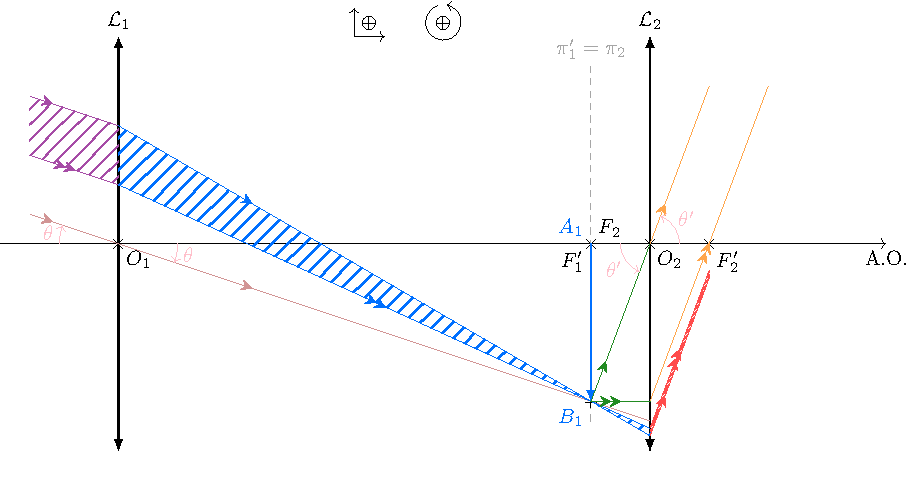
\includegraphics[width=\linewidth]{kepler.pdf}
	\end{center}
}%

\QR{%
	Calculer le grossissement de la lunette.
}{%
	~
	\begin{tcbraster}[raster columns=6, raster equal height=rows]
		\begin{tcolorbox}[blankest, raster multicolumn=1, space to=\myspace]
			\begin{tcbraster}[raster columns=1]
				\begin{tcn}[add to natural height=\myspace, valign=top](ques)
					{Résultat}
					\[
						G
					\]
				\end{tcn}
				\begin{tcn}(tool){Outil}
					\[
						G = \frac{\theta'}{\theta}
					\]
				\end{tcn}
			\end{tcbraster}
		\end{tcolorbox}
		\begin{tcn}[raster multicolumn=2](appl)""{Application}
			Avec le tracé sur le schéma et en considérant des petits angles,
			$\DS \theta' = \frac{\ABb}{\obar{O_2F_2}} > 0$ et $\DS \theta =
				\frac{\ABb}{\obar{O_1F_1'}} < 0$, soit \[ G = \frac{f_1'}{-f_2'} = -8\]
		\end{tcn}
		\begin{tcn}[raster multicolumn=3](ror)"impo"'r'{Attention}
			Pour bien voir si un angle est positif ou négatif, il faut se donner un
			sens dans lequel compter positivement, tracer les angles depuis l'axe
			optique jusqu'au rayon pour voir le changement de direction et dans la
			formule trigonométrique utiliser les grandeurs dans le bon sens.
		\end{tcn}
	\end{tcbraster}
}%

\QR{\label{q:k_cercleo}%
	Rappeler la définition du cercle oculaire et son intérêt.
}{%
	~
	\begin{tcbraster}[raster columns=2, raster equal height=rows]
		\begin{tcn}(data){Cercle oculaire}
			On appelle cercle oculaire l'image de la monture de l'objectif donnée par
			l'oculaire.
		\end{tcn}
		\begin{tcn}*(inte)"left"'r'{Utilité du cercle oculaire}
			Il correspond à la section la plus étroite du faisceau sortant de
			l'oculaire, où l'œil reçoit le maximum de lumière.
		\end{tcn}
	\end{tcbraster}
}%

\QR{%
	Déterminer sa position $\obarr{O_2C'_K}$.
}{%
	~
	\begin{tcbraster}[raster columns=6, raster equal height=rows]
		\begin{tcolorbox}[blankest, raster multicolumn=3, space to=\myspacee]
			\begin{tcbraster}[raster columns=1]
				\begin{tcn}[raster multicolumn=1,
						add to natural height=\myspacee](ques){Résultat attendu}
					$$\obarr{O_2C_K'}$$
				\end{tcn}
				\begin{tcn}[raster multicolumn=2](tool){Outil du cours}
					Par définition, C$_K'$ est l'image de O$_1$ par $\Lc_2$. On va
					donc se servir de la relation de conjugaison d'une lentille
					mince~:
					\[
						\frac{1}{\OFp} = \frac{1}{\OAp} - \frac{1}{\OA}
					\]
				\end{tcn}
			\end{tcbraster}
		\end{tcolorbox}
		\begin{tcn}[raster multicolumn=3](appl)'r'{Application}
			On a ici $\rm O \equiv O_2$, $\rm F' \equiv F_2'$, $\rm A \equiv O_1$ et
			$\rm A' \equiv C_K'$. On a donc~:
			\[
				\frac{1}{\obarr{O_2F_2'}} =
				\frac{1}{\obarr{O_2C_K'}} -
				\frac{1}{\obarr{O_2O_1}}
			\]
			et après calculs~:
			\[
				\boxed{\obarr{O_2C_K'} =
					\left[
						\frac{1}{\obarr{O_2O_1}} +
						\frac{1}{\obarr{O_2F_2'}}
						\right]^{-1} =
					\xul{\SI{+4.5}{cm}}
				}
			\]
		\end{tcn}
	\end{tcbraster}
}%

\QR{\label{q:k_diam}%
	Donner sa taille (diamètre $\rm D'_K$).
}{%
	~
	\begin{tcbraster}[raster columns=6, raster equal height=rows]
		\begin{tcolorbox}[blankest, raster multicolumn=3]
			\begin{tcbraster}[raster columns=1]
				\begin{tcn}[raster multicolumn=1](ques){Résultat attendu}
					\[D_K'\]
				\end{tcn}
				\begin{tcn}[raster multicolumn=2](tool){Outil du cours}
					Le diamètre du cercle oculaire s'apparente à la taille d'un
					objet. On peut donc utiliser le grandissement~:
					\[
						\g =
						\frac{\ABp}{\AB} =
						\frac{\OAp}{\OA}
					\]
				\end{tcn}
			\end{tcbraster}
		\end{tcolorbox}
		\begin{tcn}[raster multicolumn=3](appl)'r'{Application}
			Avec les données de l'énoncé, on obtient~:
			\[
				\g =
				\frac{D_K'}{D} =
				\frac{\obarr{O_2C_K'}}{\obarr{O_2O_1}}
			\]
			et finalement
			\[
				\boxed{D_K' = D\times \frac{\obar{O_2C_K'}}{\obar{O_2O_1}} =
					\xul{\SI{3.75}{mm}}
				}
			\]
		\end{tcn}
	\end{tcbraster}
}%


\subsection{Galilée}

\enonce{%
	On obtient une lunette de Galilée en remplaçant l'oculaire convergent par un
	oculaire divergent. Dans cet exercice, la valeur de la vergence est la même
	que précédemment en valeur absolue. On nomme cette lentille $\Lc_3$, son
	centre sera noté O$_3$. La lunette astronomique reste afocale.
}%

\QR{%
	Expliquer que la vergence de l'oculaire sera $V_3 = \SI{-25}{\delta}$.
}{%
	Si l'oculaire est divergent, cela signifie que $C_3 < 0$. On a donc $C_3 = -
		C_2$, d'où le résultat demandé.
}%

\QR{%
	Calculer le nouvel encombrement $\obarr{O_1O_3}$.
}{%
	On reprend la question \ref{q:k_encomb}, avec cette fois des indices «~3~»
	au lieu des indices «~2~», et on obtient~:

	\begin{tcbraster}[raster columns=2, raster equal height=rows]
		\begin{tcn}(appl){Application}

			$\obarr{O_1O_3} = \obarr{O_1F_1'} + \obarr{F_3O_3}$
			avec
			$\obarr{F_3O_3} = \obarr{O_3F_3'} = \SI{-4}{cm}$,
			d'où
			$\xul{\obarr{O_1O_3} = \SI{+28}{cm}}$

		\end{tcn}
		\begin{tcn}*(inte)"left"'r'{Intérêt}
			La lunette de Galilée est donc plus compacte que la lunette de Kepler !
		\end{tcn}
	\end{tcbraster}
	% \vfill
}%

\QR{%
	Tracer, toujours à l'échelle, le même schéma que précédemment avec
	cette nouvelle situation.
}{%
	\begin{center}
		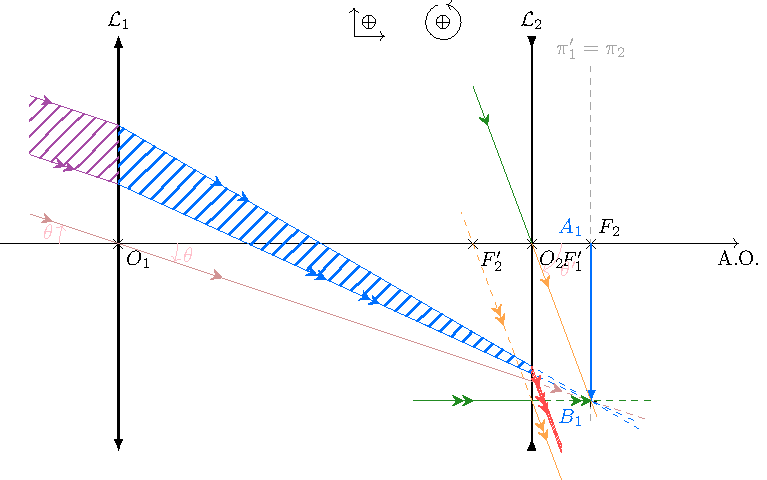
\includegraphics[width=\linewidth]{galilee.pdf}
	\end{center}
}%

\QR{%
	Déterminer la position $\obarr{O_3C'_G}$ du cercle oculaire.
}{%
	On reprend la question \ref{q:k_cercleo}, avec des indices « 3 » au lieu de
	« 2 », et on obtient~:
	\begin{tcbraster}[raster columns=3, raster equal height=rows]
		\begin{tcn}[raster multicolumn=1](appl){Application}
			\[
				\xul{\obarr{O_3C_G'} = \SI{-3.5}{cm}}
			\]
		\end{tcn}
		\begin{tcn}[raster multicolumn=2](rema)"lrem"'r'{Comparaison}
			On a cette fois un cercle oculaire virtuel. Il faudra placer son œil le
			plus près possible de l'oculaire pour espérer avoir le plus de lumière
			possible.
		\end{tcn}
	\end{tcbraster}
}%

\QR{%
	Donner sa taille (diamètre $D'\ind{G}$).
}{%
	On reprend la question \ref{q:k_diam}~:
	\begin{center}
		\begin{tcn}(appl){Application}
			\[
				\xul{D_G' = \SI{3.75}{mm}}
			\]
		\end{tcn}
	\end{center}
}%

\QR{%
	Quels sont les avantages et inconvénients de ces 2 lunettes
	astronomiques~?
}{%
	\begin{center}
		\begin{tabularx}{.7\linewidth}{|Y*{2}{|Y}|}\hline
			\rowcolor{gray!15}                  & Avantages                              & Inconvénients \\\hline
			\cellcolor{gray!15} Lunette Galilée & + compacte\smallbreak image droite     &
			cercle oculaire virtuel                                                                      \\\hline
			\cellcolor{gray!15} Lunette Kepler  & Grande clarté \smallbreak Cercle
			oculaire réel                       & - compacte \smallbreak image renversée                 \\\hline
		\end{tabularx}
	\end{center}
}%

\end{document}
